\subsubsection{UC\theuccount-SE - Consumer Email inoltra il messaggio finale al server Email}
%	\begin{figure}[H]
%		\centering
%		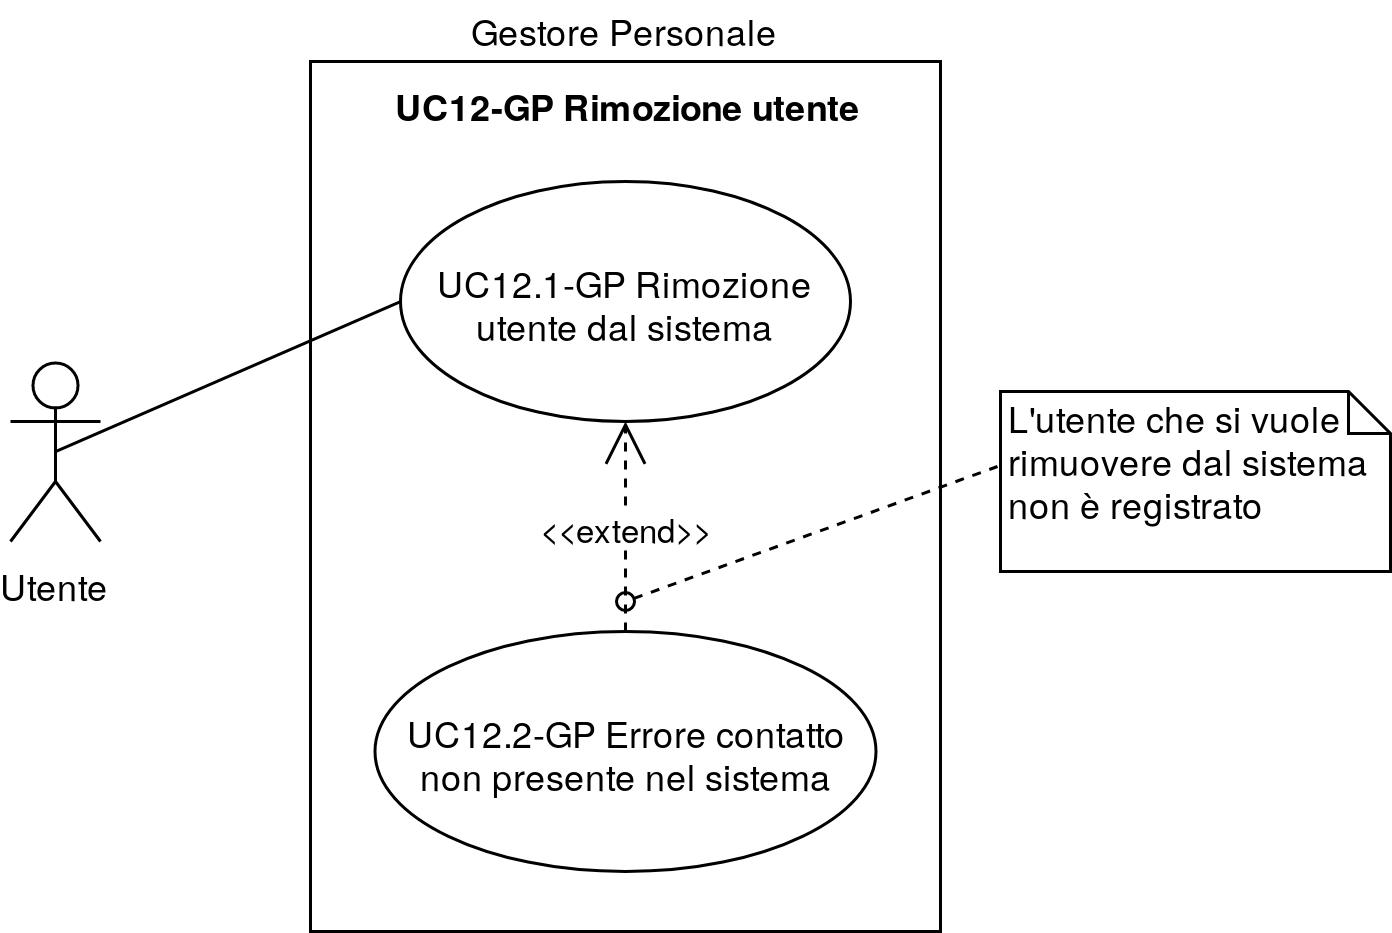
\includegraphics[width=0.8\textwidth]{img/casi_d'uso/UC12.png}\\
%		\caption{UC\theuccount-SE - Consumer Email inoltra il messaggio finale al server Email}
%	\end{figure}
	\begin{itemize}
		\item \textbf{Codice}: UC\theuccount-SE.
		\item \textbf{Titolo}: Consumer Email inoltra il messaggio finale al server Email.
		\item \textbf{Attori primari}: Consumer Email.
		\item \textbf{Descrizione}: il Consumer Email inoltra il messaggio finale al server Email, il quale notifica il destinatario finale attraverso una Email.
		\item \textbf{Precondizione}: il Consumer Email ha ricevuto almeno un messaggio.
		\item \textbf{Postcondizione}: il server Email ha ricevuto il messaggio finale con successo.
		\item \textbf{Scenario principale}: 
		\begin{enumerate}
			\item Il Consumer Email riceve un messaggio dal Gestore Personale
			\item Il Consumer Email procede all'inoltro del messaggio finale al server Email
		\end{enumerate}
		
	\end{itemize}